Kap. 19, s. 617-652
+ notater på nett

\subsection{Oppbygning}
En bipolar junction transistor bruker både elektron- og hullstrøm,
og har 2 \emph{junctions} mellom ulikt dopede halvledere.
BJTer kommer i 2 typer, NPN og PNP. Vi skal se på den første av dem.

\paragraph{Collector, Base og Emittor} \mbox{} \\
En BJT består av 3 deler: collector, base og emittor.
Disse er bygget opp av tre dopede halvleder materialer, n-type og p-type.
Mellom disse regionene er pn-overganger akkurat som i dioder. \\\\
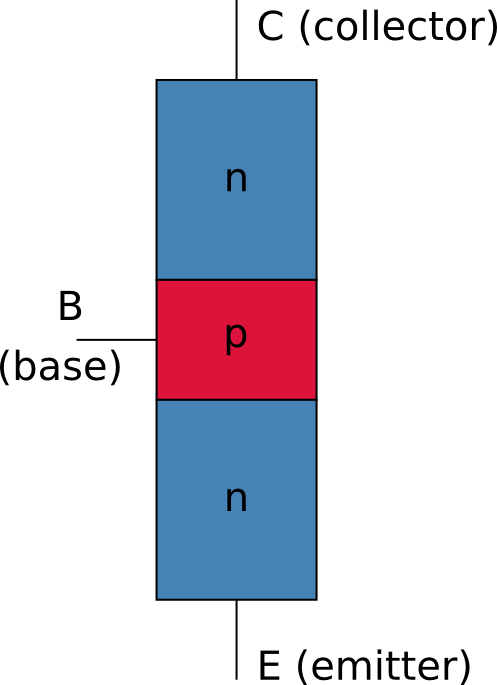
\includegraphics[width=0.5\textwidth]{./img/npn}
\\\\
Symbolet for BJTer ser slik ut for npn \\\\
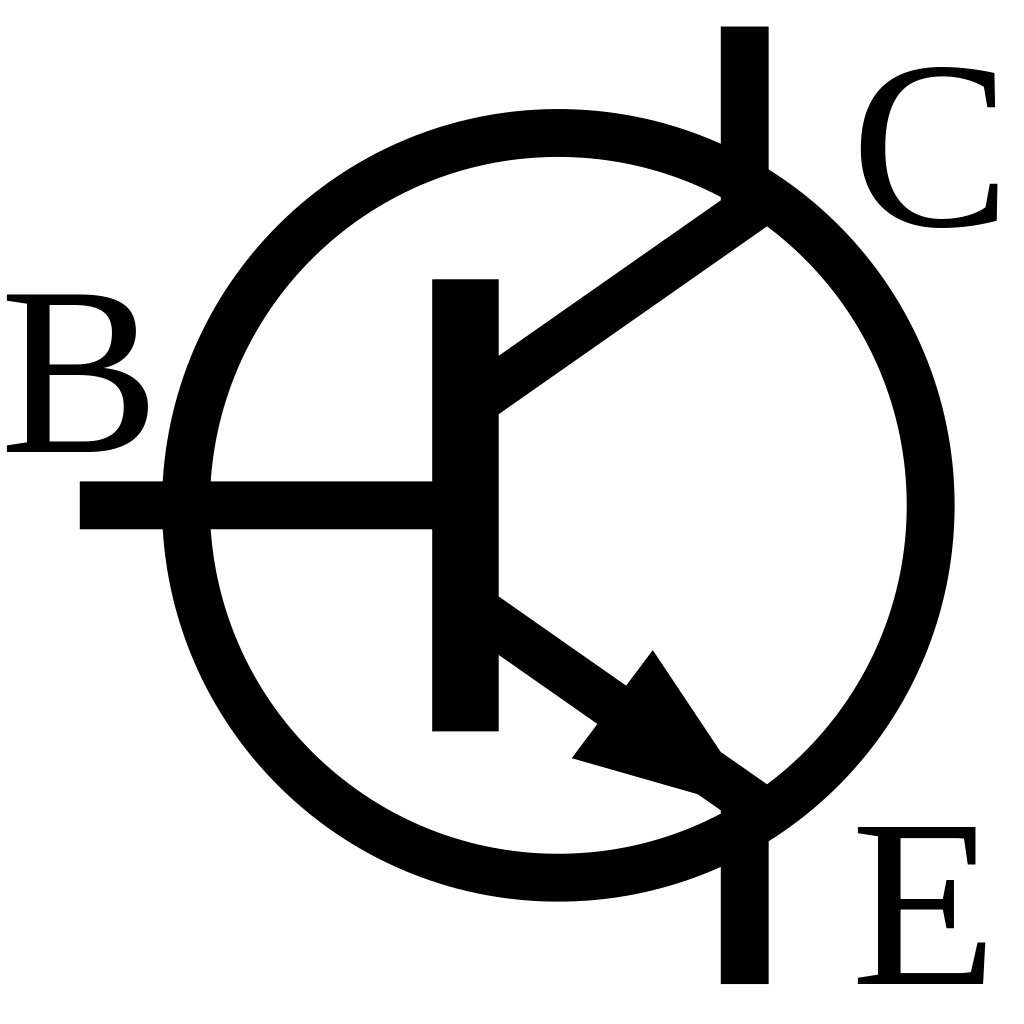
\includegraphics[width=0.25\textwidth]{./img/npn-symbol} \\
Hvor den lille pilen peker mot det n-dopede materialet.
\\
Tilsvarende for pnp \\\\
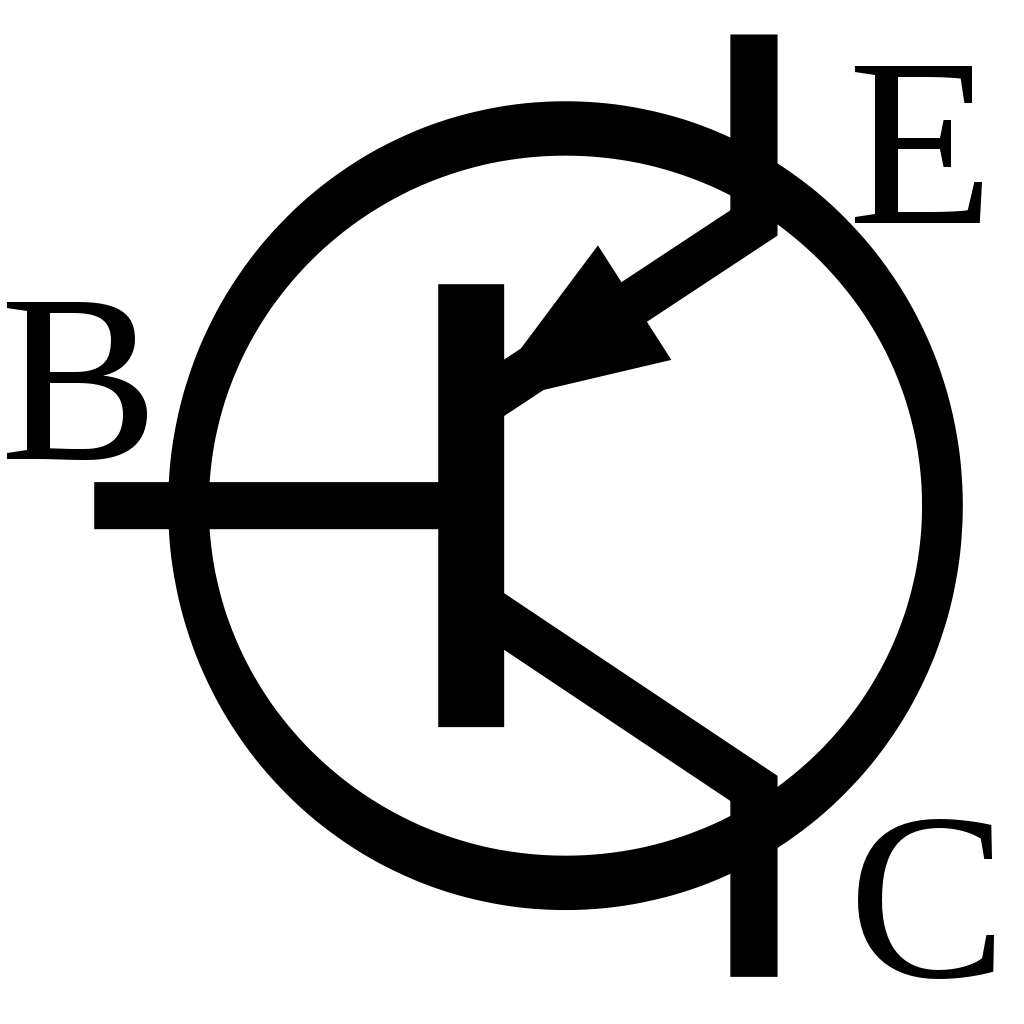
\includegraphics[width=0.25\textwidth]{./img/pnp-symbol}


\paragraph{Fysisk struktur} \mbox{} \\
I virkeligheten er en BJT bygget opp lag på lag med en isolator rundt.
\\\\
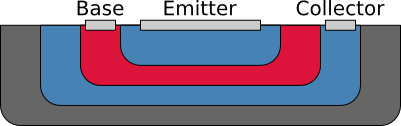
\includegraphics{./img/npn-real}


\subsection{Virkemåte}
  \subsubsection{Operasjonsmodi}
    Siden NPN-transistoren består av 2 PN-overganger,
kan man anse det som to dioder koblet sammen.
\\\\
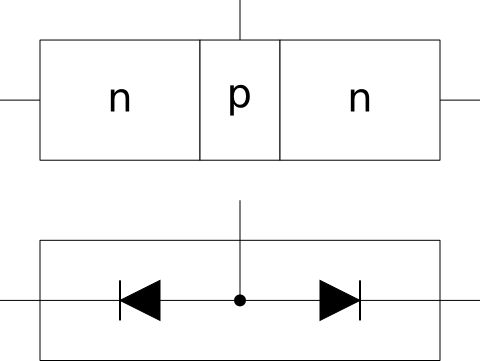
\includegraphics[width=0.5\textwidth]{./img/npn-bias}
\\\\
Disse diodene kan kjøres i forskjellig bias (forward, reverse).
Avhengig av forholdet mellom spenningen
ved diodens collector, base og emitter, fungerer transistoren forskjellig.

De forskjellige kombinasjonene utgjør transistorens operasjonsmodi.
\\\\
\begin{tabular}{ l | c | r}
Base-Emitter & Base-Collector & Operasjonsmodi \\ \hline
Reverse & Reverse & Cutoff \\
Forward & Reverse & Aktiv \\
Forward & Forward & Metning \\
\end{tabular}

  \subsubsection{Cutoff modus}
    Både base-emitter junction og collector-base junction
er i reverse bias.
Vi vet fra hvordan dioder fungerer at sperresjiktet
mellom de dopede materialene vokser.
I cutoff modus fungerer transistoren som en åpen krets,
ingen strøm passerer gjennom.
\\\\
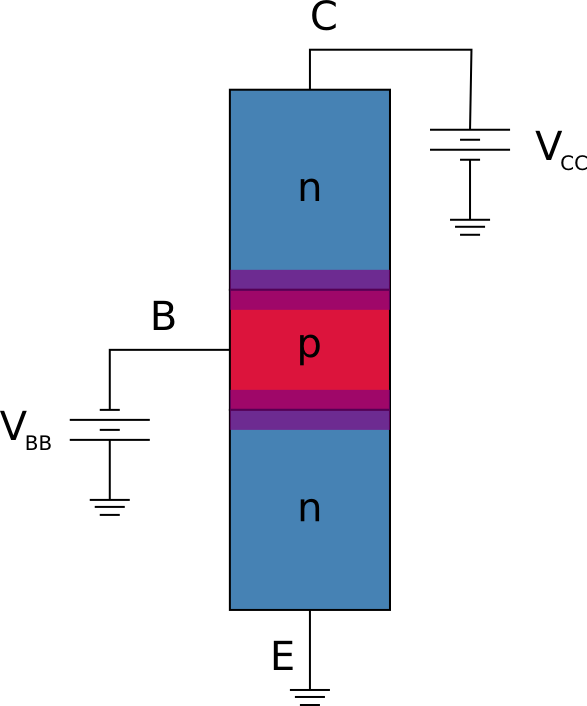
\includegraphics[width=0.5\textwidth]{./img/npn-cutoff}

  \subsubsection{Metning}
    Når spenningen ved basen er større enn ved collector,
fungerer transistoren som en kortslutning.
Strøm går fra emitter til collector.
\\\\
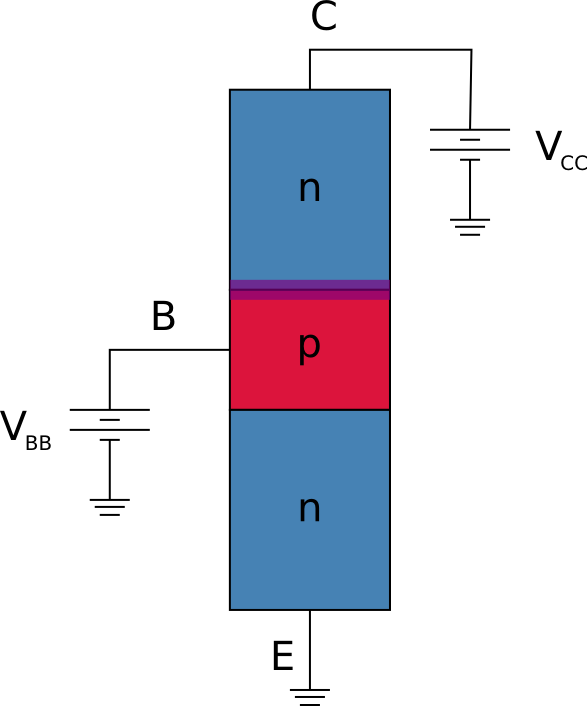
\includegraphics[width=0.5\textwidth]{./img/npn-metning}

lederetning \\
basen tynn, diffusjon, minoritetsbærere \\
depletion layer og strøm til kollektor \\
(med illustrasjoner) \\
Hans table av modi \\
4 squares of modi \\
TODO

\subsection{Karakteristikk}
Strømforhold ligning (aktiv modus?) og symbol
Virkeområde
Temperatureffekt
TODO
